\documentclass[tikz,border=6pt]{standalone}
\usepackage{amsmath}
\definecolor{cG}{RGB}{31,94,165}\definecolor{cX}{RGB}{214,96,33}
\tikzset{
  dot/.style={circle,inner sep=0pt,minimum size=3.2pt,fill=black!22},
  ch/.style={circle,inner sep=0pt,minimum size=8pt,ball color=cG!55,draw=cG!80!black,line width=0.3pt},
  fp/.style={circle,inner sep=0pt,minimum size=8pt,ball color=cX!45,draw=cX!80!black,line width=0.3pt},
  arr/.style={-{Stealth[length=4pt]},line width=0.6pt,black!65},
  lay/.style={line width=0.4pt,black!25,fill=black!3,fill opacity=0.55},
  vl/.style={font=\small,inner sep=1pt}}
\usetikzlibrary{arrows.meta}
\begin{document}
% K_{2,2,2} x H_21 as six stacked copies of H_21, one for each vertex of the octahedron (layer g at
% depth g). Blue: the vertices (j mod 3, j) of the sequence; orange: their footprints
% (x_{(j+1) mod 3}, j); each arrow joins a vertex to its footprint in the same column j.
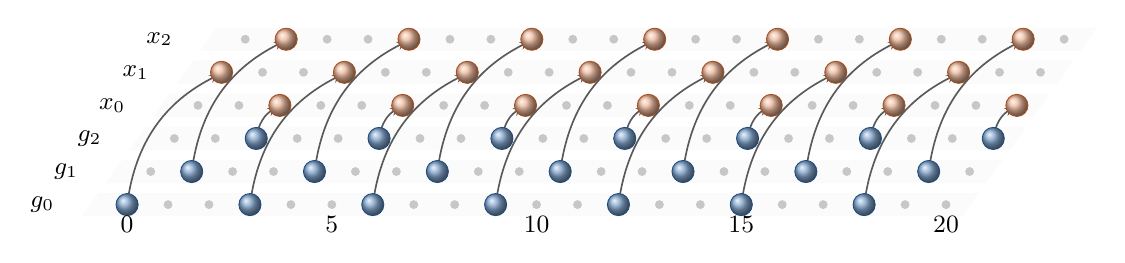
\begin{tikzpicture}[x={(0.52cm,0cm)},y={(0.30cm,0.42cm)},z={(0cm,1cm)},line cap=round]
\foreach \g in {5,4,...,0}{
  \fill[lay] (-0.9,\g-0.35,0) -- (20.6,\g-0.35,0) -- (20.6,\g+0.35,0) -- (-0.9,\g+0.35,0) -- cycle;
  \foreach \h in {0,...,20}{\node[dot] at (\h,\g,0) {};}
  \pgfmathtruncatemacro{\x}{\g-3}
  \ifnum\g<3 \node[vl,anchor=east] at (-1.7,\g,0) {$g_{\g}$};\else\node[vl,anchor=east] at (-1.7,\g,0) {$x_{\x}$};\fi}
\foreach \j in {0,...,20}{
  \pgfmathtruncatemacro{\t}{mod(\j,3)}\pgfmathtruncatemacro{\f}{mod(\j+1,3)+3}
  \draw[arr] (\j,\t,0) to[bend left=28] (\j,\f-0.05,0);
  \node[fp] at (\j,\f,0) {};
  \node[ch] at (\j,\t,0) {};}
\foreach \h in {0,5,10,15,20}{\node[vl,below=3pt] at (\h,0,0) {$\h$};}
\end{tikzpicture}
\end{document}
